\documentclass{jhwhw}

\title{Tutorial B5B\\Applications of Differentiation}
\author{Eytan Chong}
\date{2024-04-04}

\begin{document}
    \problem{}
        The equation of a closed curve is $(x+2y)^2 + 3(x-y)^2 = 27$.

        \begin{enumerate}
            \item Show, by differentiation, that the gradient at the point $(x,y)$ on the curve may be expressed in the form $\der{y}{x} = \dfrac{y-4x}{7y-x}$.
            \item Find the equations of the tangents to the curve that are parallel to
            \begin{enumerate}
                \item the $x$-axis,
                \item the $y$-axis.
            \end{enumerate}
        \end{enumerate}

    \solution
        \part
            Implicitly differentiating the given equation,

            \begin{alignat*}{2}
                &&2(x+2y)\left(1 + 2y^\prime\right) + 6(x-y)(1 - y^\prime) &= 0\\
                &&(x+2y)\left(1 + 2y^\prime\right) + 3(x-y)(1 - y^\prime) &= 0\\
                \implies&& x + 2xy^\prime + 2y + 4y\cdot y^\prime + 3x - 3x\cdot y^\prime - 3y + 3y\cdot y^\prime &= 0\\
                \implies&& (-x + 7y)y^\prime + 4x - y &= 0\\
                \implies&& y^\prime &= \dfrac{y-4x}{7y-x}
            \end{alignat*}

        \part
            \subpart
                When the tangent to the curve is parallel to the $x$-axis, $y^\prime = 0$.

                \begin{alignat*}{2}
                    &&y^\prime &= 0\\
                    \implies&&\dfrac{y-4x}{7y-x} &= 0\\
                    \implies&&y-4x &= 0\\
                    \implies&&y &= 4x
                \end{alignat*}

                Substituting $y=4x$ into the given equation,

                \begin{alignat*}{2}
                    &&(x+2 \cdot 4x)^2 + 3(x-4x)^2 &= 27\\
                    &&(9x)^2 + 3(-3x)^2 &= 27\\
                    &&81x^2 + 27x^2 &= 27\\
                    &&108x^2 &= 27\\
                    &&x^2 = \dfrac14\\
                    &&x = \pm \dfrac12
                \end{alignat*}

                Hence, $y = \pm 2$. Since the tangents to the curve is parallel to the $x$-axis, the equation of the tangents is $y = \pm 2$.

                \boxt{
                    $y = \pm 2$
                }

            \subpart
                When the tangent to the curve is parallel to the $y$-axis, $y^\prime$ is undefined. Hence, $7y-x =0 \implies x = 7y$. Substituting $x = 7y$ into the given equation,

                \begin{alignat*}{2}
                    &&(7y+2y)^2 + 3(7y-y)^2 &= 27\\
                    &&(9y)^2 + 3(6y)^2 &= 27\\
                    &&81y^2 + 108y^2 &= 27\\
                    &&189y^2 &= 27\\
                    &&y^2 &= \dfrac17\\
                    &&y &= \pm \dfrac1{\sqrt7}\\
                \end{alignat*}

                Hence, $x = \pm \dfrac{7}{\sqrt7} = \pm \sqrt7$. Since the tangents to the curve is parallel to the $y$-axis, the equation of the tangents is $x = \pm \sqrt7$.

                \boxt{
                    $x = \pm \sqrt7$
                }

    \problem{}
        A piece of wire of length 8 cm is cut into two piece, one of length $x$ cm, the other of length $(8-x)$ cm. The piece of length $x$ cm is bent to form a circle with circumference $x$ cm. The other piece is bent to form a square with perimeter $(8-x)$ cm. Show that, as $x$ varies, the sum of the areas enclosed by these two pieces of wire is a minimum when the radius of the circle is $\dfrac4{4+\pi}$ cm.

    \solution
        Let the radius of the circle be $r$ cm. Then we have $x = 2\pi r \implies r = \dfrac{x}{2\pi}$. Let the side length of the square be $s$ cm. Then we have $8-x=4s \implies s = 2-\dfrac{x}4$.

        Let the total area enclosed by the circle and the square be $A(x)$.

        \begin{align*}
            A(x) &= \pi r^2 + s^2\\
            &= \pi \left(\dfrac{x}{2\pi}\right)^2 + \left(2-\dfrac{x}4\right)^2\\
            &= \dfrac1{4\pi}x^2 + \left(4 - x + \dfrac1{16}x^2\right)\\
            &= \left(\dfrac1{4\pi} + \dfrac1{16}\right)x^2 - x + 4
        \end{align*}

        Consider the stationary points of $A(x)$. For stationary points, $A^\prime(x) = 0$.

        \begin{alignat*}{2}
            &&A^\prime(x) &= 0\\
            \implies&&\left(\dfrac1{4\pi} + \dfrac1{16}\right)\cdot 2x - 1 &= 0\\
            \implies&&\left(\dfrac1{2\pi} + \dfrac1{8}\right)x - 1 &= 0\\
            \implies&& x &= \dfrac1{\tfrac1{2\pi} + \tfrac1{8}}\\
            && &= \dfrac{16\pi}{8 + 2\pi}\\
            && &=\dfrac{8\pi}{4 + \pi}
        \end{alignat*}

        \begin{table}[h]
            \centering
            \begin{tabular}{|c|c|c|c|}
            \hline
            $x$ & $\left(\dfrac{8\pi}{4 + \pi}\right)^-$ & $\dfrac{8\pi}{4 + \pi}$ & $\left(\dfrac{8\pi}{4 + \pi}\right)^+$ \\\hline
            $\der{A}{x}$ & -ve   & 0 & +ve   \\[1ex]\hline
            \end{tabular}
        \end{table}

        Hence, the minimum value of $A(x)$ is achieved when $x = \dfrac{8\pi}{4 + \pi}$, whence $r = \dfrac{1}{2\pi} \cdot \dfrac{8\pi}{4 + \pi} = \dfrac{4}{4+\pi}$ cm.

    \problem{}
        A spherical balloon is being inflated in such a way that its volume is increasing at a constant rate of 150 cm$^3$s$^{-1}$. At time $t$ seconds, the radisu of the balloon is $r$ cm.

        \begin{enumerate}
            \item Find $\der{r}{t}$ when $r = 50$.
            \item Find the rate of increase of the surface area of the baloon when its radius is 50 cm.
        \end{enumerate}

    \solution
        Let the volume of the balloon be $V(r) = \dfrac43 \pi r^3$ cm$^3$.

        \part
            Note that $\der{V}{t} = 150$ and $\der{V}{r} = 4\pi r^2$. 

            \begin{align*}
                \der{r}{t} &= \der{r}{V} \cdot \der{V}{t}\\
                &= \left(\der{V}{r}\right)^{-1} \cdot \der{V}{t}\\
                &= \dfrac1{150} \cdot 4 \pi r^2\\
                &= \dfrac{75}{2\pi r^2}
            \end{align*}

            Evaluating $\der{r}{t}$ at $r=50$,

            \begin{align*}
                \left.\der{r}{t}\right|_{r=50} &= \dfrac{75}{2 \pi \cdot 50^2}\\
                &= \dfrac3{200\pi}
            \end{align*}

            \boxt{
                When $r = 50$, $\der{r}{t} = \dfrac3{200\pi}$
            }

        \part
            Let the surface area of the balloon be $A(r) = 4\pi r^2$. Observe that $\der{A}{r} = 8 \pi r$.

            \begin{alignat*}{2}
                &&\der{A}{t} &= \der{A}{r} \cdot \der{r}{t}\\
                &&\left.\der{A}{t}\right|_{r=50} &= \left.\left(\der{A}{r} \cdot \der{r}{t}\right)\right|_{r=50}\\
                && &= 8\pi\cdot50 \cdot \dfrac3{200\pi}\\
                && &= 6
            \end{alignat*}

            \boxt{
                The rate of increase of the surface area of the balloon when its radius is 50 cm is 6 cm/s.
            }

    \problem{}
        A curve has parametric equations $x = 5\sec\theta, \, y = 3\tan\theta$, where $-\dfrac12\pi < \theta < \dfrac12\pi$. Find the exact coordinates of the point on the curve at which the normal is parallel to the line $y=x$.

    \solution
        Observe that $x^2 = 25\sec^2\theta$ and $\dfrac{25}9 y^2 = 25\tan^2\theta$. Using the identity $\tan^2\theta + 1 = \sec^2\theta$,

        \begin{equation}\label{P4-1}
            \dfrac{25}9 y^2 + 25 = x^2
        \end{equation}

        Implicitly differentiating, we get $\dfrac{25}9 \cdot 2y \cdot y^\prime = 2x \implies \dfrac{25}9 \cdot y \cdot y^\prime = x$.

        Since the normal is parallel to $y =x$, the tangent is perpendicular is perpendicular to $y=x$. Hence, the tangent is parallel to $y = -x$, whence $y^\prime = -1$.

        \begin{alignat*}{2}
            \dfrac{25}9 \cdot y \cdot -1 &= x\\
            y = -\dfrac{9}{25} x
        \end{alignat*}

        Substituting $y = -\dfrac9{25}x$ into Equation~\ref{P4-1},

        \begin{alignat*}{2}
            &&\dfrac{25}9 \left(-\dfrac9{25}x\right)^2+25 &= x^2\\
            \implies&&\dfrac{9}{25} + 25 &= x^2\\
            \implies&&\dfrac{16}{25}x^2 &= 25\\
            \implies&&\left(\dfrac45 x\right)^2 &= 5^2\\
            \implies&&\dfrac45 x &= \pm 5\\
            \implies&& x &= \pm \dfrac{25}4
        \end{alignat*}

        Observe that for $-\dfrac12\pi < \theta < \dfrac12\pi$, $x=5\sec\theta \geq 5$. We thus reject $x = -\dfrac{25}4$. Hence, $x=\dfrac{25}4$, whence $y = -\dfrac{9}{25} \cdot \dfrac{25}4 = -\dfrac{9}4$. The coordinate of the required point is thus $\left(\dfrac{25}4, -\dfrac94\right)$.
        
        \boxt{
            $\left(\dfrac{25}4, -\dfrac94\right)$
        }

    \problem{}
        The parametric equations of a curve are

        \begin{equation}
            x = t^2, \, y = \dfrac2t
        \end{equation}

        \begin{enumerate}
            \item Find the equation of the tangent to the curve at the point $(p^2, \dfrac2p)$, simplifying your answer.
            \item Hence find the coordinates of the points $Q$ and $R$ where this tangent meets the $x$- and $y$-axes respectively.
            \item The point $F$ is the mid-point of $QR$. Find a Cartesian equation of the curve traced by $F$ as $p$ varies.
        \end{enumerate}

    \solution
        \part
            Observe that $\der{x}{t} = 2t$ and $\der{y}{t} = -\dfrac{2}{t^2}$.

            \begin{align*}
                \der{y}{x} &= \der{y}{t} \cdot \der{t}{x} \\
                &= \der{y}{t} \cdot \left(\der{x}{t}\right)^2\\
                &= -\dfrac{2}{t^2} \cdot \dfrac1{2t}\\
                &= -\dfrac1{t^3}
            \end{align*}

            At the point $p^2, \dfrac2p$, $t = p$, whence $\der{y}{x} = -\dfrac{1}{p^3}$. Using the point-slope formula, the tangent to the curve is given by the equation
            
            \begin{alignat*}{2}
                &&y - \dfrac2p &= -\dfrac1{p^3}\left(x - p^2\right)\\
                \implies&&y &= \dfrac{2}p -\dfrac1{p^3}\left(x - p^2\right)\\
                && &= \dfrac{2}p -\dfrac1{p^3}x + \dfrac1p\\
                && &= \dfrac{3}p -\dfrac1{p^3}x
            \end{alignat*}

            \boxt{
                $y = \dfrac{3}p -\dfrac1{p^3}x$
            }

        \part
            \case{1}{$y = 0$}
                \begin{alignat*}{2}
                    &&0 &= \dfrac{3}p -\dfrac1{p^3}x\\
                    \implies&&\dfrac1{p^3}x &= \dfrac3p\\
                    \implies&&x &= 3p^2
                \end{alignat*}

                Hence, $Q(3p^2, 0)$.

            \case{2}{$x = 0$}
                \begin{align*}
                    y &= \dfrac{3}p -\dfrac1{p^3}\cdot0\\
                    &= \dfrac3p
                \end{align*}

                Hence, $R\left(0, \dfrac3p\right)$.

            \boxt{
                $Q(3p^2, 0)$, $R\left(0, \dfrac3p\right)$
            }

        \part
            \begin{align*}
                F &= \left(\dfrac12 \cdot 3p^2, \dfrac12 \cdot \dfrac3p\right)\\
                &= \left(\dfrac32 p^2, \dfrac3{2p}\right)
            \end{align*}

            As $p$ varies, $F$ traces a curve given by the parametric equations $x = \dfrac32 p^2$, $y = \dfrac3{2p}$. Observe that $p = \dfrac3{2y}$.

            \begin{alignat*}{2}
                &&x &= \dfrac32 \left(\dfrac3{2y}\right)^2\\
                && &= \left(\dfrac32\right)^3 \dfrac1{y^2}\\
                \implies&&y^2 &= \left(\dfrac32\right)^3 \dfrac1x\\
                \implies&&y &= \pm\sqrt{\left(\dfrac32\right)^3  \dfrac1x}\\
                \implies&&y &= \pm \left(\dfrac32\right)^{\tfrac32}  \dfrac1{\sqrt{x}}
            \end{alignat*}

            \boxt{
                $y = \pm \left(\dfrac32\right)^{\tfrac32}  \dfrac1{\sqrt{x}}$
            }

    \problem{}
        \begin{center}
            \begin{tikzpicture}
                \draw (0,0) arc[x radius=2, y radius=2, start angle=180, end angle=0];

                \draw (0, 0) -- (0, -2);

                \draw (4, 0) -- (4, -2);

                \draw (0, -2) -- (4, -2);

                \draw[dotted, thick] (0, 0) -- (4, 0);

                \node[anchor=east] at (0, -1) {$y$};

                \node[anchor=north] at (2, -2) {$x$};
            \end{tikzpicture}    
        \end{center}
        
        \noindent A new flower-bed is being designed for a large garden. The flower-bed will occupy a rectangle $x$ m by $y$ m together with a semicircle of diameter $x$ m, as shown in the diagram. A low wall will be built around the flowerbed. The time needed to build the wall will be 3 hours per metre for the straight parts and 9 hours per metre for the semicircular part. Given that a total time of 180 hours is taken to build the wall, find, using differentiation, the values of $x$ and $y$ which give a flower-bed of maximum area.

    \solution
        Observe that the length of the straight parts is $(2y + x)$ m, while the length of the semicicular part is $\dfrac12 \cdot 2\pi\left(\dfrac{x}2\right) = \dfrac12 \pi x$ m. Since a total time of 180 hours is taken to build the wall,

        \begin{alignat*}{2}
            &&3 (2y + x) + 9\left(\dfrac12 \pi x\right) &= 180\\
            \implies&& (2y + x) + 3\left(\dfrac12 \pi x\right) &= 60\\
            \implies&&2y + x + \dfrac32 \pi x &= 60\\
            \implies&&4y + 2x + 3\pi x &= 120\\
            \implies&&(2 + 3\pi)x &= 120-4y\\
            \implies&& x &= \dfrac{120-4y}{2+3\pi}
        \end{alignat*}

        Let $A(y)$ be the total area enclosed by the garden, in m$^2$. Observe that $A(y) = xy + \dfrac12 \pi \left(\dfrac{x}2\right)^2 = xy + \dfrac18 \pi x^2$. Also note that $x^\prime = -\dfrac4{2 + 3\pi}$. Now, consider the stationary points of $A(y)$. For stationary points, $A^\prime(y) = 0$.

        \begin{alignat*}{2}
            &&A^\prime(y) &= 0\\
            \implies&&\left(x^\prime y + x\right) + \dfrac18 \pi (2x \cdot x^\prime) &= 0\\
            \implies&&x^\prime y + x + \dfrac14 \pi (x \cdot x^\prime) &= 0
        \end{alignat*}

        Substituting $x = \dfrac{120-4y}{2+3\pi}$ and $x^\prime = -\dfrac4{2 + 3\pi}$,

        \begin{alignat*}{2}
            &&-\dfrac4{2 + 3\pi} \cdot y + \dfrac{120-4y}{2+3\pi} + \dfrac14 \pi \left(\dfrac{120-4y}{2+3\pi} \cdot -\dfrac4{2 + 3\pi}\right) &= 0\\
            \implies&&-4 \cdot y + (120-4y) + \dfrac14 \pi \left(\dfrac{120-4y}{2+3\pi} \cdot -4\right) &= 0\\
            \implies&&120 - 8y - \pi \left(\dfrac{120-4y}{2+3\pi}\right) &= 0\\
            \implies&&120(2+3\pi) - 8(2+3\pi)y - \pi(120-4y) &= 0\\
            \implies&&240 + 360\pi - 16y - 24\pi y - 120\pi + 4\pi y &= 0\\
            \implies&&240 + 240\pi - 16y - 20\pi y &= 0\\
            \implies&&60 + 60\pi - 4y - 5\pi y &= 0\\
            \implies&& 4y + 5\pi y &= 60 + 60\pi\\
            \implies&& (4 + 5\pi)y &= 60 + 60\pi\\
            \implies&& y &= \dfrac{60 + 60\pi}{4 + 5\pi}\\
        \end{alignat*}

        Using the equation $x = \dfrac{120-4y}{2 + 3\pi}$, 

        \begin{align*}
            x &= \dfrac{120-4\cdot\tfrac{60 + 60\pi}{4 + 5\pi}}{2 + 3\pi}\\
            &= \dfrac{120(4+5\pi) - 4(60 + 60\pi)}{(2+3\pi)(4+5\pi)}\\
            &= \dfrac{480 + 600\pi - 240 -240\pi}{(2+3\pi)(4+5\pi)}\\
            &= \dfrac{240 + 360\pi}{(2+3\pi)(4+5\pi)}\\
            &= \dfrac{120 (2 + 3\pi)}{(2+3\pi)(4+5\pi)}\\
            &= \dfrac{120}{4+5\pi}
        \end{align*}

        \boxt{
            $x = \dfrac{120}{4+5\pi}$, $y = \dfrac{60 + 60\pi}{4 + 5\pi}$
        }

    \problem{}
        \begin{center}
            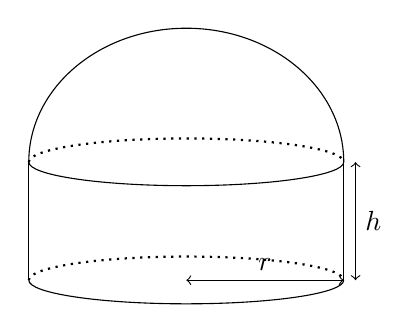
\begin{tikzpicture}
                \draw (0,0) arc[x radius=2, y radius=1.7, start angle=180, end angle=0];

                \draw (0, 0) arc[x radius=2, y radius=0.3, start angle=-180, end angle=0];

                \draw[dotted, thick] (0, 0) arc[x radius=2, y radius=0.3, start angle=180, end angle=0];

                \draw (0, 0) -- (0, -1.5);

                \draw (4, 0) -- (4, -1.5);

                \draw (0, -1.5) arc[x radius=2, y radius=0.3, start angle=-180, end angle=0];

                \draw[dotted, thick] (0, -1.5) arc[x radius=2, y radius=0.3, start angle=180, end angle=0];

                \draw[<->] (2, -1.5) -- (4, -1.5);

                \node[anchor=south] at (3, -1.5) {$r$};

                \draw[<->] (4.15, 0) -- (4.15, -1.5);

                \node[anchor=west] at (4.15, -0.75) {$h$};
            \end{tikzpicture}    
        \end{center}

        \noindent A model of a concert hall is made up of three parts.

        \begin{itemize}
            \item The roof is modelled by the curved surface of a hemisphere of radius $r$ cm.
            \item The walls are modelled by the curved surface of a cylinder of radius $r$ cm and height $h$ cm.
            \item The floor is modelled by a circular disc of radius $r$ cm.
        \end{itemize}

        \noindent The three parts are joined together as shown in the diagram. The model is made of material of negligible thickness.

        \begin{enumerate}
            \item It is given that the volume of the model is a fixed value $k$ cm$^3$, and the external surface area is a minimum. Use differentiation to find the values of $r$ and $h$ in terms of $k$. Simplify your answers.
            \item It is given instead that the volume of the model is 200 cm$^3$ and its external surface area is 180 cm$^2$. Show that there are two possible values of $r$. Given also that $r < h$, find the value of $r$ and the value of $h$.
        \end{enumerate}

    \solution
        \part
            Let the volume of the model be $V$ cm$^3$. Then
            \begin{alignat}{2}
                V = &&\dfrac12 \cdot \dfrac43 \pi r^3 + \pi r^2 h &= k\label{P7-1}\\
                \implies&&\dfrac23 r+h &= \dfrac{k}{\pi r^2}\nonumber\\
                \implies&&h &= \dfrac{k}{\pi r^2}-\dfrac23 r\label{P7-2}
            \end{alignat}

            Let the external surface area of the model be $A$ cm$^2$. Then
            \begin{align}
                A &= \dfrac12 \cdot 4\pi r^2 + 2\pi r h + \pi r^2\nonumber\\
                &= 3\pi r^2 + 2\pi rh\nonumber\\
                &= 3\pi r^2 + 2\pi r\left(\dfrac{k}{\pi r^2}-\dfrac23 r\right)\nonumber\\
                &= 3\pi r^2 + \dfrac{2k}{r}-\dfrac43 \pi r^2\nonumber\\
                &= \dfrac53\pi r^2 + \dfrac{2k}{r}\label{P7-3}
            \end{align}

            Consider the stationary points of $A$. For stationary points, $\der{A}{r} = 0$.
            \begin{alignat*}{2}
                &&\der{A}r &= 0\\
                \implies&&\dfrac53\pi \cdot 2r - \dfrac{2k}{r^2} &= 0\\
                \implies&&\dfrac{5}3\pi r^3 - k &= 0\\
                \implies&&r^3 &= \dfrac{3k}{5\pi}\\
                \implies&&r &= \sqrt[3]{\dfrac{3k}{5\pi}}
            \end{alignat*}

            \begin{table}[h]
                \centering
                \begin{tabular}{|c|c|c|c|}
                \hline
                $r$ & $\sqrt[3]{\dfrac{3k}{5\pi}}^-$ & $\sqrt[3]{\dfrac{3k}{5\pi}}$ & $\sqrt[3]{\dfrac{3k}{5\pi}}^+$ \\\hline
                $\der{A}{r}$ & -ve   & 0 & +ve   \\[1ex]\hline
                \end{tabular}
            \end{table}

            Hence, $A$ is at a minimum when $r = \sqrt[3]{\dfrac{3k}{5\pi}}$.

            Substituting $r = \sqrt[3]{\dfrac{3k}{5\pi}}$ into Equation~\ref{P7-1},

            \begin{alignat*}{2}
                &&\dfrac23 \pi \left(\dfrac{3k}{5\pi}\right) + \pi r^2 h &= k\\
                \implies&&\dfrac{2}{5}k + \pi r^2h &= k\\
                \implies&&\pi r^2 h &= \dfrac{3}{5}k\\
                \implies&&r^2 h &= \dfrac{3k}{5\pi}\\
                \implies&&r^2 h &= r^3\\
                \implies&&h &= r\\
                && &= \sqrt[3]{\dfrac{3k}{5\pi}}
            \end{alignat*}

            \boxt{
                $r = \sqrt[3]{\dfrac{3k}{5\pi}}$, $h = \sqrt[3]{\dfrac{3k}{5\pi}}$
            }

        \part
            From Equation~\ref{P7-3}, we have
            \begin{alignat*}{2}
                &&\dfrac53\pi r^2 + \dfrac{2\cdot200}{r} &= 180\\
                \implies&&\dfrac53\pi r^2 + \dfrac{400}{r} - 180 &= 0\\
                \implies&&\dfrac53\pi r^3 - 180r + 400  &= 0\\
                \implies&&\pi r^3 - 108r + 240 &= 0
            \end{alignat*}

            Let $f(r) = \pi r^3 - 108r + 240$. Consider the stationary points of $f(r)$. For stationary points, $f^\prime(r) = 0$.            
            \begin{alignat*}{2}
                &&f^\prime(r) &= 0\\
                \implies&&3\pi r^2 - 108 &= 0\\
                \implies&& r^2 &= \dfrac{36}{\pi}
            \end{alignat*}

            Hence, $r = \pm \sqrt{\dfrac{36}{\pi}} = \pm \dfrac6{\sqrt\pi}$. Consider the case when $r= \dfrac6{\sqrt\pi}$.

            \begin{table}[h]
                \centering
                \begin{tabular}{|c|c|c|c|}
                \hline
                $r$ & $\dfrac6{\sqrt\pi}^-$ & $\dfrac6{\sqrt\pi}$ & $\dfrac6{\sqrt\pi}^+$ \\\hline
                $f^\prime(r)$ & -ve   & 0 & +ve   \\\hline
                \end{tabular}
            \end{table}

            Hence, $f(r)$ attains a minimum when $r = \dfrac6{\sqrt\pi}$. Since $f\left(\dfrac6{\sqrt\pi}\right) < 0$ and $f(0) > 0$, there exist positive $r_1$ and  $r_2$ such that $r_1 < r_2$ and $f(r_1) = f(r_2) = 0$. There are hence two possible values of $r$, which are $3.04$ and $3.72$ respectively.

            From Equation~\ref{P7-2}, we know that $h= \dfrac{200}{\pi r^2} - \dfrac23 r$. When $r = 3.04$, $h = 4.88 > r$. When $r = 3.72$, $h = 2.12 < r$. Thus, given that $r < h$, $r = 3.04$ and $h = 4.88$.

            \boxt{
                $r = 3.04$, $h = 4.88$
            }

    \problem{}
        \begin{center}
            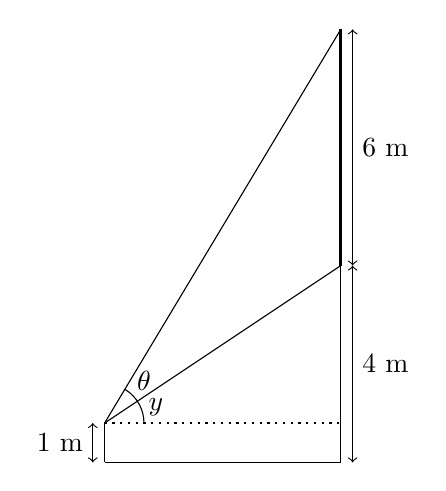
\begin{tikzpicture}
                \draw[dotted, thick] (0, 0) -- (3, 0);

                \draw (3, 0) -- (3, 2);

                \draw[very thick] (3, 2) -- (3, 5);

                \draw (0, 0) -- (3, 5);

                \draw (0, 0) -- (3, 2);

                \draw (0, 0) -- (0, -0.5);

                \draw (0, -0.5) -- (3, -0.5);

                \draw (3, -0.5) -- (3, 0);

                \draw[<->] (3.15, -0.5) -- (3.15, 2);

                \node[anchor=west] at (3.15, 0.75) {4 m};

                \draw[<->] (3.15, 2) -- (3.15, 5);

                \node[anchor=west] at (3.15, 3.5) {6 m};

                \draw[<->] (-0.15, 0) -- (-0.15, -0.5);

                \node[anchor=east] at (-0.15, -0.25) {1 m};

                \draw (0.5, 0) arc[x radius=0.5, y radius=0.5, start angle=0, end angle=59];

                \node at (0.65, 0.2) {$y$};

                \node at (0.5, 0.53) {$\theta$};
            \end{tikzpicture}
        \end{center}
        
        \noindent A movie screen on a vertical wall is 6 m high and 4 m above the horizontal floor. A boy who is standing at $x$ m away from the wall has eye level at 1 m above the floor as shown in the diagram.

        The viewing angle of the boy at that position is $\theta$ and the angle of elevation of the bottom of the screen is $y$.

        \begin{enumerate}
            \item Express $y$ in terms of $x$.
            \item By expressing $\theta$ in terms of $x$ or otherwise, find the stationary value of $\theta$, giving your answers in exact form. Determine if the value is a maximum or minimum value, showing your working clearly.
        \end{enumerate}

    \solution
        \part
            Observe that $\tan y = \dfrac3x$, whence $y = \arctan \dfrac3x$.

            \boxt{
                $y = \arctan \dfrac3x$
            }

        \part
            Observe that $\tan (y + \theta) = \dfrac9x$. 

            \begin{alignat*}{2}
                &&\tan (y + \theta) &= \dfrac9x\\
                \implies&&\dfrac{\tan y + \tan \theta}{1 - \tan y \tan \theta} &= \dfrac9x\\
                \implies&&\dfrac{\tfrac3x + \tan \theta}{1 - \tfrac3x \tan \theta} &= \dfrac9x\\
                \implies&&\dfrac{3 + x\tan \theta}{x - 3\tan \theta} &= \dfrac9x\\
                \implies&&x(3 + x\tan \theta) &= 9(x - 3\tan \theta)
            \end{alignat*}
            \begin{alignat*}{2}
                \implies&&3x + x^2\tan\theta &= 9x - 27 \tan \theta\\
                \implies&&x^2\tan\theta + 27 \tan \theta &= 6x \\
                \implies&&(x^2 + 27)\tan\theta&= 6x\\
                \implies&&\tan\theta &= \dfrac{6x}{x^2+27}
            \end{alignat*}

            Implicitly differentiating,
            \begin{alignat*}{2}
                &&\sec^2(\theta)\cdot\theta^\prime &= \dfrac{(x^2+27)\cdot 6 - 6x \cdot 2x}{(x^2+27)^2}\\
                \implies&&\theta^\prime&=\dfrac{-6x^2 + 162}{(x^2+27)^2\sec^2\theta}
            \end{alignat*}

            Using the identity $\tan^2 \theta + 1 = \sec^2\theta$, we have $\sec^2\theta = \left(\dfrac{6x}{x^2+27}\right)^2 + 1$.

            \begin{align*}
                \theta^\prime &= \dfrac{-6x^2 + 162}{(x^2+27)^2\left(\left(\dfrac{6x}{x^2+27}\right)^2 + 1\right)}\\
                &= \dfrac{-6x^2 + 162}{(6x)^2 + \left(x^2+27\right)^2}\\
                &= \dfrac{-6x^2 + 162}{36x^2 + \left(x^2+27\right)^2}
            \end{align*}

            For stationary points, $\theta^\prime = 0$. Hence,
            \begin{alignat*}{2}
                &&-6x^2 + 162 &= 0\\
                \implies&&x^2 &= 27\\
                \implies&&x &= \pm \sqrt{27}
            \end{alignat*}

            Since $x > 0$, we only take $x = \sqrt{27}=3\sqrt{3}$. Thus, $\tan\theta = \dfrac3{3\sqrt{3}} = \dfrac1{\sqrt3}$, whence $\theta = \dfrac{\pi}{6}$.

            \boxt{
                $\theta = \dfrac{\pi}6$
            }

            \begin{table}[h]
                \centering
                \begin{tabular}{|c|c|c|c|}
                \hline
                $x$ & $\sqrt{27}^-$ & $\sqrt{27}$ & $\sqrt{27}^+$ \\\hline
                $\theta^\prime$ & +ve   & 0 & -ve   \\\hline
                \end{tabular}
            \end{table}

            Thus, by the First Derivative Test, $\theta = \dfrac{\pi}6$ is a maximum value.

            \boxt{
                $\theta=\dfrac{\pi}6$ is a maximum value.
            }

    \problem{}
        \begin{center}
            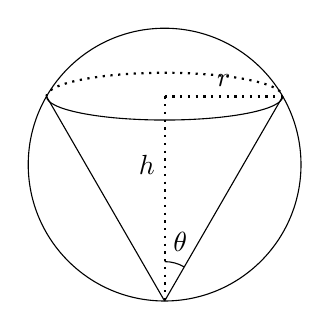
\begin{tikzpicture}
                \draw (0, 0) circle[radius=sqrt(3)];

                \draw (-1.5, 0.5*sqrt 3) arc[x radius=1.5, y radius=0.3, start angle=-180, end angle=0];

                \draw[dotted, thick] (-1.5, 0.5*sqrt 3) arc[x radius=1.5, y radius=0.3, start angle=180, end angle=0];

                \draw (-1.5, 0.5*sqrt 3) -- (0, -sqrt 3);

                \draw (1.5, 0.5*sqrt 3) -- (0, -sqrt 3);

                \draw[dotted, thick] (0, 0.5*sqrt 3) -- (1.5, 0.5*sqrt 3);

                \node[anchor=south] at (0.75, 0.5*sqrt 3) {$r$};

                \draw[dotted, thick] (0, 0.5*sqrt 3) -- (0, -sqrt 3);

                \node[anchor=east] at (0, 0) {$h$};

                \draw (0, 0.5-sqrt 3) arc[x radius=0.5, y radius=0.5, start angle=90, end angle=60];

                \node at (0.20, 0.75-sqrt 3) {$\theta$};
            \end{tikzpicture}    
        \end{center}

        \noindent The diagram shows a right inverted cone of radius $r$, height $h$ and semi-vertical angle $\theta$, which is inscribed in a sphere of radius 1 unit.

        Prove that $r^2 = 2h - h^2$.

        \begin{enumerate}
            \item As $r$ and $h$ varies, determine the exact maximum volume of the cone.
            \item Show that $h = 2\cos^2\theta$. The volume of the cone is increasing at a rate of 6 unit$^3$/s when $h = \dfrac32$. Determine the rate of change of $\theta$ at this instant, leaving your answer in an exact form.
        \end{enumerate}

    \solution
        Consider the following diagram of the cone and sphere.

        \begin{center}
            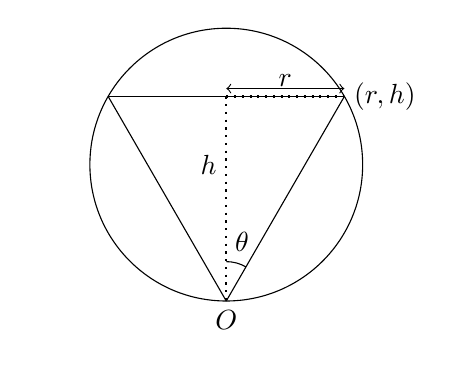
\begin{tikzpicture}
                \draw (0, 0) circle[radius=sqrt(3)];

                \draw (-1.5, 0.5*sqrt 3) -- (1.5, 0.5*sqrt 3);

                \draw (-1.5, 0.5*sqrt 3) -- (0, -sqrt 3);

                \draw (1.5, 0.5*sqrt 3) -- (0, -sqrt 3);

                \draw[dotted, thick] (0, 0.5*sqrt 3) -- (1.5, 0.5*sqrt 3);

                \draw[<->] (0, 0.5 * sqrt 3 + 0.1) -- (1.5, 0.5*sqrt 3 + 0.1);

                \node[anchor=south] at (0.75, 0.5*sqrt 3) {$r$};

                \draw[dotted, thick] (0, 0.5*sqrt 3) -- (0, -sqrt 3);

                \node[anchor=east] at (0, 0) {$h$};

                \draw (0, 0.5-sqrt 3) arc[x radius=0.5, y radius=0.5, start angle=90, end angle=60];

                \node at (0.20, 0.75-sqrt 3) {$\theta$};

                \node[anchor=north] at (0, -sqrt 3) {$O$};

                \node[anchor=west] at (1.5, 0.5 *sqrt 3) {$(r, h)$};

                \node[anchor=east, white] at (-1.5, 0.5 *sqrt 3) {$(r, h)$};
            \end{tikzpicture}    
        \end{center}

        Let the origin be the tip of the cone. Since the sphere has radius 1 unit, the circle is given by the equation $x^2 + (y-1)^2 = 1$. Since the point $(r, h)$ lies on the circle,
        \begin{alignat}{2}
            &&r^2 + (h-1)^2 &= 1\nonumber\\
            \implies&&r^2 + h^2 - 2h + 1 &= 1\nonumber\\
            \implies&&r^2 &= 2h - h^2\label{P9-1}
        \end{alignat}

        \part

            Implicitly differentiating Equation~\ref{P9-1},
            \begin{alignat*}{2}
                &&2r &= 2h^\prime - 2h\cdot h^\prime\\
                \implies&&r &= h^\prime - h\cdot h^\prime\\
                && &= h^\prime (1 - h)\\
                \implies&& h^\prime &= \dfrac{r}{1 - h}
            \end{alignat*}

            Let the volume of the cone be $V(r) = \dfrac13 \pi r^2 h$. Differentiating $V(r)$,
            \begin{align*}
                V^\prime(r) &= \dfrac13 \pi (r^2 h^\prime + h \cdot 2r)\\
                &= \dfrac13 \pi \left(\left(2h - h^2\right)\left(\dfrac{r}{1-h}\right) + 2hr\right)\\
                &= \dfrac13 \pi \left(hr\cdot\dfrac{2 - h}{1-h} + 2hr\right)\\
                &= \dfrac13 \pi rh \left(\dfrac{2 - h}{1-h} + 2\right)\\
                &= \dfrac13 \cdot \dfrac{\pi rh}{1-h}(2 - h + 2(1-h))\\
                &= \dfrac13 \cdot \dfrac{\pi rh}{1-h}(2 - h + 2-2h)\\
                &= \dfrac13 \cdot \dfrac{\pi rh}{1-h}(4-3h)
            \end{align*}

            Consider the stationary values of $V(r)$. For stationary values, $V^\prime(r) = 0$.
            \begin{alignat*}{2}
                &&V^\prime(r) &= 0\\
                \implies&& \dfrac13 \cdot \dfrac{\pi rh}{1-h}(4-3h) &= 0\\
                \implies&& 4-3h &= 0\\
                \implies&& h &= \dfrac43
            \end{alignat*}

            Substituting $h = \dfrac43$ into Equation~\ref{P9-1}, we obtain $r^2 = 2\cdot\dfrac43 - \left(\dfrac43\right)^2  = \dfrac89$, whence $r = \dfrac{2\sqrt2}3$ (we reject $r = -\dfrac{2\sqrt2}3$ as $r > 0$).

            \begin{table}[h]
                \centering
                \begin{tabular}{|c|c|c|c|}
                \hline
                $r$ & $\dfrac{2\sqrt2}3^-$ & $\dfrac{2\sqrt2}3$ & $\dfrac{2\sqrt2}3^+$ \\[1ex]\hline
                $V^\prime(r)$ & +ve   & 0 & -ve   \\\hline
                \end{tabular}
            \end{table}

            Hence, the maximum volume is indeed achieved when $r =\dfrac{2\sqrt2}3$. 

            \begin{align*}
                V\left(\dfrac{2\sqrt2}3\right) &= \dfrac13 \pi \cdot \dfrac89 \cdot \dfrac43\\
                &= \dfrac{32}{81}\pi
            \end{align*}

            \boxt{
                The maximum volume of the cone is $\dfrac{32}{81} \pi$ units$^3$.
            }

        \part
            From the diagram, we see that $\cos\theta = \dfrac{h}{\sqrt{r^2 + h^2}}$.

            \begin{alignat*}{2}
                &&\cos\theta &= \dfrac{h}{\sqrt{r^2 + h^2}}\\
                \implies&&\cos^2\theta &= \dfrac{h^2}(r^2 + h^2)\\
                \implies&&2\cos^2\theta &= \dfrac{2h^2}{r^2 + h^2}\\
                && &= \dfrac{2h^2}{2h-h^2+h^2}\\
                && &= \dfrac{2h^2}{2h}\\
                && &= h
            \end{alignat*}
            \begin{alignat*}{2}
                &&2\cos^2\theta - 1 &= h - 1\\
                \implies&&\cos 2\theta &= h-1\\
                \implies&&\cos^2 2\theta &= (h-1)^2\\
                \implies&&\sin^2 2\theta &= 1-(h-1)^2\\
                \implies&&\sin 2\theta &= \pm \sqrt{1-(h-1)^2}
            \end{alignat*}

            Since $0 < \theta < \dfrac{\pi}2$, we know $\sin 2\theta > 0$. We thus take $\sin 2\theta = \sqrt{1 - (h-1)^2}$.
            
            Implicitly differentiating $2\cos^2\theta = h$ with respect to $h$,

            \begin{alignat*}{2}
                &&2\cdot 2 \cos\theta \cdot -\sin\theta \cdot \der{\theta}{h} &= 1\\
                \implies&&\der{\theta}h &= \dfrac{1}{-4\sin\theta\cos\theta}\\
                && &= \dfrac1{-2\sin 2\theta}\\
                && &= \dfrac1{-2 \sqrt{1 - (h-1)^2}}
            \end{alignat*}
            \begin{align*}
                \der{\theta}{t} &= \der{\theta}h \cdot \der{h}r \cdot \der{r}V \cdot \der{V}t\\
                &= \der{\theta}h \cdot \der{h}r \cdot \left(\der{V}r\right)^{-1} \cdot \der{V}t\\
                &= \dfrac1{-2 \sqrt{1 - (h-1)^2}} \cdot \dfrac{r}{1-h} \cdot \left(\dfrac13 \cdot \dfrac{\pi rh}{1-h} (4-3h) \right)^{-1} \cdot \der{V}t\\
                &= \dfrac1{-2 \sqrt{1 - (h-1)^2}} \cdot \dfrac{r}{1-h} \cdot 3 \cdot \dfrac{1-h}{\pi rh(4-3h)}  \cdot \der{V}t\\
                &= \dfrac3{\pi} \cdot \dfrac1{-2 \sqrt{1 - (h-1)^2}} \cdot \dfrac1{h(4-3h)}  \cdot \der{V}t
            \end{align*}

            Evaluating $\der{\theta}t$ at $h = \dfrac32$,

            \begin{align*}
                \left.\der{\theta}t\right|_{h = \tfrac32} &= \dfrac3{\pi} \cdot \dfrac1{-2 \sqrt{1 - (\tfrac32-1)^2}} \cdot \dfrac1{\tfrac32(4-3\cdot\tfrac32)}  \cdot 6\\
                &= \dfrac{18}{\pi} \cdot -\dfrac1{\sqrt{3}} \cdot -\dfrac43\\
                &= \dfrac{24}{\pi} \cdot \dfrac{\sqrt 3}{3}\\
                &= \dfrac{8\sqrt{3}}{\pi}
            \end{align*}

            Hence, $\theta$ is increasing at a rate of $\dfrac{8\sqrt3}{\pi}$ radians per second when $h = \dfrac32$.

            \boxt{
                $\dfrac{8\sqrt3}{\pi}$ rad/s
            }

    \problem{}
        \begin{center}
            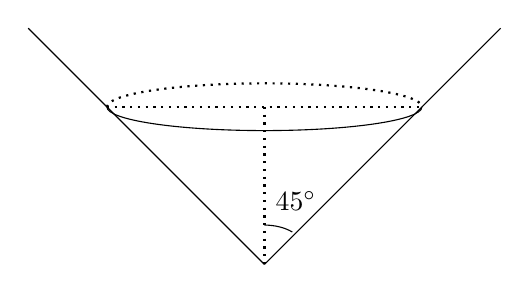
\begin{tikzpicture}
                \draw (0, 0) -- (-3, 3);

                \draw (0, 0) -- (3, 3);

                \draw(-2, 2) arc[x radius=2, y radius=0.3, start angle=-180, end angle=0];
                
                \draw[dotted, thick] (-2, 2) arc[x radius=2, y radius=0.3, start angle=180, end angle=0];

                \draw[dotted, thick] (-2, 2) -- (2, 2);

                \draw[dotted, thick] (0, 2) -- (0, 0);

                \draw (0, 0.5) arc[x radius=0.5, y radius=0.3, start angle=90, end angle=45];

                \node at (0.4, 0.8) {$45^\circ$};
            \end{tikzpicture}    
        \end{center}

        \noindent A hollow cone of semi-vertical angle $45^\circ$ is held with its axis vertical and vertex downwards. At the beginning of an experiment, it is follows with 390 cm$^3$ of liquid. The liquid runs out thorugh a small hole at the vertex at a constant rate of 2 cm$^3$/s. 

        Find the rate at which the depth of the liquid is decreasing 3 minutes after the start of the experiment.

    \solution
        Consider the following diagram.

        \begin{center}
            \begin{tikzpicture}
                \draw (0, 0) -- (-3, 3);

                \draw (0, 0) -- (3, 3);

                \draw (-2, 2) -- (2, 2);

                \draw[dotted, thick] (0, 2) -- (0, 0);

                \draw (0, 0.5) arc[x radius=0.5, y radius=0.3, start angle=90, end angle=45];

                \node at (0.4, 0.8) {$45^\circ$};

                \node[anchor=east] at (0, 1.25) {$h$};

                \node[anchor=south] at (1, 2) {$r$};

                \draw[<->] (0, 2.1) -- (2, 2.1); 
            \end{tikzpicture}    
        \end{center}

        Let the volume of liquid be $V$ cm$^3$. From the diagram, we have $r = h$. Thus,

        \begin{equation*}
            V = \dfrac13 \pi h^3
        \end{equation*}

        Differentiating $V$ with respect to $h$,

        \begin{align*}
            \der{V}{h}&= \dfrac13 \pi \cdot 3 h^2\\
            &= \pi h^2
        \end{align*}

        Let $t$ be time in seconds. Consider $\der{h}t$.

        \begin{align*}
            \der{h}t &= \der{h}V \cdot \der{V}t\\
            &= \left(\der{h}V\right)^{-1} \cdot \der{V}t\\
            &= \dfrac1{\pi h^2} \cdot -2\\
            &= \dfrac{-2}{\pi h^2}
        \end{align*}

        When $t = 180$, there is $390 - 180\cdot2 = 30$ cm$^3$ of liquid left in the cone.
        \begin{alignat*}{2}
            &&V &= 30\\
            \implies&&\dfrac13 \pi h^3 &= 30\\
            \implies&&h^3 &= \dfrac{90}{\pi}\\
            \implies&&h &= \sqrt[3]{\dfrac{90}{\pi}}
        \end{alignat*}

        Evaluating $\der{h}{t}$ at $t =180$,

        \begin{align*}
            \left.\der{h}t\right|_{t = 180} &= \left.\der{h}t\right|_{h = \sqrt[3]{\tfrac{90}{\pi}}}\\
            &= \dfrac{-2}{\pi \left(\sqrt[3]{\tfrac{90}{\pi}}\right)^2}\\
            &= -0.0680 \tosf{3}
        \end{align*}

        \boxt{
            The depth of the liquid is decreasing at a rate of 0.0680 cm/s 3 minutes after the start of the experiment.
        }


    \problem{}
        A particle is projected from the origin $O$ and it moes freely under gravity in the $x$-$y$ plane. At time $t$ s after projection, the particle is at the point $(x,y)$ where $x=30t$ and $y=20t-5t^2$, with $x$ and $y$ measured in meteres.

        \begin{enumerate}
            \item Given that the particle passes through two points $A$ and $B$ which are at a distance 15 m above the $x$-axis, find the time taken for the particle to travel from $A$ to $B$. Find also the distance $AB$.
            \item It is known that the particle always travels in a direction tangential to its path. Show that, when $x=10$, the particle is travelling at an angle of $\arctan \dfrac59$ above the horizontal.
            
            The speed of the particle is given by $\sqrt{\left(\der{x}{t}\right)^2 + \left(\der{y}{t}\right)^2}$. Find the speed of the particle when $x = 10$.
            \item Show that the equation of trajectory is $y = \dfrac23 x - \dfrac1{180} x^2$.
        \end{enumerate}
        
    \solution
        \part
            Consider $y = 15$.

            \begin{alignat*}{2}
                &&y &= 15\\
                &&20t-5t^2&=15\\
                &&t^2-4t+3&=0\\
                &&(t-1)(t-3) &= 0
            \end{alignat*}

            Hence, $t = 1$ or $t = 3$. Thus, the particle takes $3-1 = 2$ seconds to travel from $A$ to $B$.

            \boxt{
                2 seconds
            }

            \smallskip

            \case{1}{$t = 1$} When $t = 1$, $x = 30\cdot1 = 30$. Thus, $A(30, 15)$.

            \case {2}{$t=3$} When $t = 3$, $x = 30\cdot3 = 90$. Thus, $B(90, 15)$.

            \smallskip

            The distance $AB$ is thus $90-30 = 60$ m.

            \boxt{
                $AB = 60$ m
            }

        \part
            Note that $\der{x}{t} = 30$ and $\der{y}t = 20-10t$. Thus

            \begin{align*}
                \der{y}{x} &= \der{y}{t} \cdot \der{t}{x}\\
                &= \der{y}t \cdot \left(\der{x}{t}\right)^{-1}\\
                &= (20 - 10t) \cdot \dfrac{1}{30}\\
                &= \dfrac{2-t}{3}
            \end{align*}

            When $x = 10$, $t = \dfrac13$. Evaluating $\der{y}{x}$ at $t = \dfrac13$,

            \begin{align*}
                \left.\der{y}{x}\right|_{t = \tfrac13} &= \dfrac{2-\tfrac13}{3}\\
                &= \dfrac59
            \end{align*}

            Hence, the line tangent to the curve at $x=10$ has gradient $\dfrac59$. Thus, the particle is travelling at an angle of $\arctan\dfrac59$ above the horizontal when $x=10$.

            \begin{align*}
                \left.\sqrt{\left(\der{x}{t}\right)^2 + \left(\der{y}{t}\right)^2}\right|_{t=\tfrac13} &= \sqrt{30^2 + (20 - \tfrac{10}3)^2}\\
                &= 34.3 \tosf{3}
            \end{align*}

            \boxt{
                The particle is travelling at a speed of 34.3 m/s when $x = 10$.
            }

        \part
            Note that $t = \dfrac{x}{30}$. Hence,
            \begin{align*}
                y &= 20t - 5t^2\\
                &= 20\cdot\dfrac{x}{30} - 5\left(\dfrac{x}{30}\right)^2\\
                &= \dfrac23 x - \dfrac1{180}x^2
            \end{align*}
\end{document}